%%%%%%%%%%%%%%%%%%%%%%%%%%%%%%%%%%%%%%%%%%%%%%%%%%%%%%%%%%%%%%%%%%% 
%                                                                 %
%                            CHAPTER                              %
%                                                                 %
%%%%%%%%%%%%%%%%%%%%%%%%%%%%%%%%%%%%%%%%%%%%%%%%%%%%%%%%%%%%%%%%%%% 
%\chapter{Structuur van de masterproeftekst}
\chapter{Herkenning en Detectie Algemeen}

\section{Deep learning-gebaseerde herkeningssystemen}
Herkeningssytemen of classificatie systemen voorspellen wat de klasse van een object is in een afbeelding. Dus het herkennen van objecten in digitale afbeeldingen zonder deze te localiseren of aan te duiden. Voor een herkenningssysteem is er een goed getraind netwerk nodig dat input afbeeldingen omzet in features. Er moet een database zijn met daarin de gegevens van de objecten die men wilt herkennen. Vervolgens hebben is er ook een methode nodig om features van het neuraal netwerk te vergelijken met de gegevens in de database om het juiste object te herkennen.

\subsection{convolutioneel neuraal netwerk (CNN) }
\begin{figure}[!ht]
    \centering
 	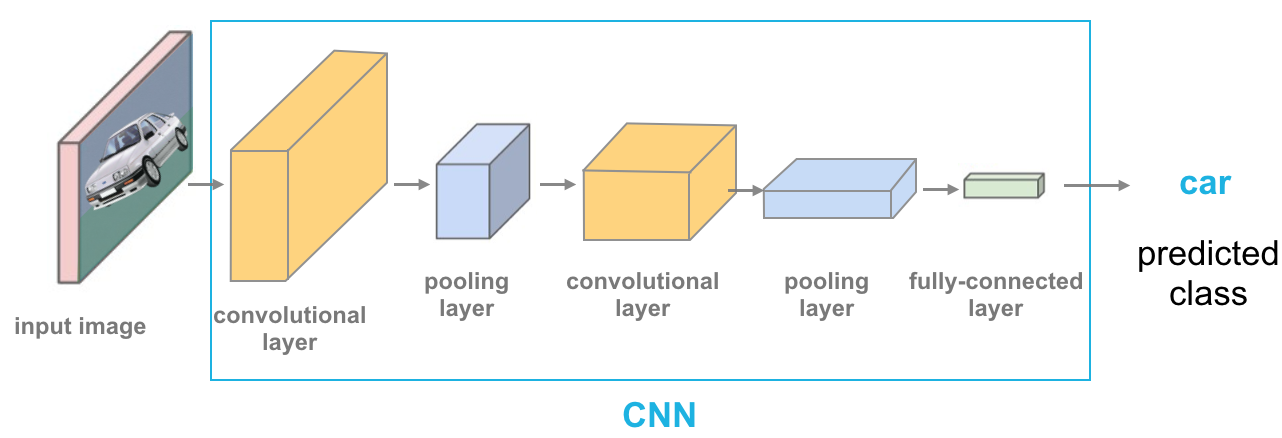
\includegraphics[width=0.80\linewidth]{fig/CNN.png}
 	\caption{CNN met 2 convolutie lagen en 2 pooling lagen en een fully-connected layer}
 	\label{fig:cnn}
\end{figure}

De belankrijkste bouwsteen van een herkenningssysteem is een goed getrainde CNN (figuur \ref{fig:cnn}). In tegenstelling tot fully connected netwerken wordt bij een CNN de gewichten gedeeld over verschillende locaties om zo het aantal parameters te verminderen.

\subsubsection{Convolutie laag}
\begin{figure}[!ht]
 	\centering
 	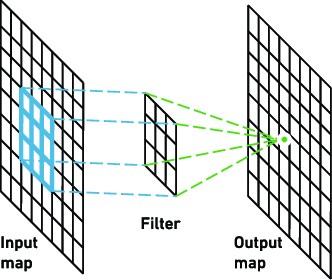
\includegraphics[width=0.35\linewidth]{fig/convolution layer.png}
 	\caption{Convolutie laag waarbij een filter wordt herleid tot een output feature.}
 	\label{fig:conv_laag}
\end{figure}
 
Het belangrijkste deel van een CNN zijn de convolutielagen (figuur \ref{fig:conv_laag}) waarbij men een kernel/filter over de input laat gaan wat als output een feature map genereerd. Een kernel bestaat uit set van gewichten die met de input worden vermenigvuldigd, deze kernel wordt over de input afbeelding geschoven. Al de pixels binnen het veld van de kernel worden gereduceert tot een enkele waarde. CNN leren verschillende features met verschillende kernels in parallel. Waardoor de matrices met feature mappen steeds kleiner worden maar ook dieper worden. Een andere factor van een convolutie laag is de stride, deze waarde geeft aan met hoeveel pixels de kernel telkens moet doorschuiven. Een CNN bestaat uit een opeenvolging van een aantal convolutie lagen die steeds meer high-level features extraheren. Hoe meer convolutielagen een netwerk telt hoe meer features er uit de input worden gehaald, maar hoe trager het netwerk is. 

\subsubsection{Lineare activatie fucntie}
Elke convolutie laag wordt gevolgd door een niet-lineare activatie functie, de meest gebruikt functie hiervoor is de rectified linear unit (ReLu) (figuur \ref{fig:relu}). De ReLu wordt vaak gebruikt omdat deze eenvoudig is, kan exact 0 weergeven en ziet er linear uit. Max(0,x) is de ReLu bewerking, dus er wordt verdergegaan met 0 of de input waarde. Zonder een niet-lineare activatie functie kan het CNN herleid worden tot 1 convolultie laag die geen high-level features kan extraheren. Andere mogelijkheden voor Lineare activatie functies zijn: Sigmoid en Tangens hyperbolicus maar deze functies vragen meer rekenwerk.

\begin{figure}[!ht]
 	\centering
 	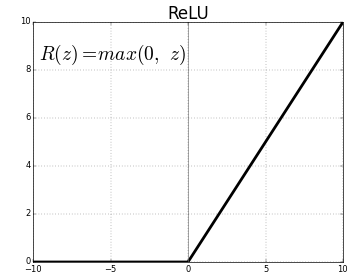
\includegraphics[width=0.35\linewidth]{fig/ReLu.png}
 	\caption{ReLu, waarbij het maximum wordt genomen van 0 en de input waarde.}
 	\label{fig:relu}
\end{figure}

\subsubsection{Pooling laag}
Een volgende bouwsteen is de pooling laag waarbij het aantal samples in de feature map wordt verlaagt. De meest voorkomende methode is max-pooling waarbij er verder wordt gegaan met de maximum waarde in een bepaalde regio. Het doel van een pooling laag is om het aantal parameters te verminderen en zo ook het rekenwerk te verminderen. Er kan ook gebruik gemaakt worden van avarage pooling waarbij er verder wordt gegaan met de gemiddelde waarde van een regio. Er is ook minimal pooling waarbij er verder wordt gegaan met de minimum waarde.

\subsubsection{Fully-connected lagen}
Op het einde van elk CNN volgen er meestal 1 of meerdere fully connected lagen. Deze lagen connecteren elke input van \'e\'en laag met elke activatie eenheid van de volgende laag. Dit zorgt voor meer parameters en meer rekenwerk waardoor deze lagen een vertragende factor vormen. De fully connected lagen gaan niet-lineare combinaties leren van de features van de convolutie lagen. De fully connected lagen zorgen voor een classificatie op basis van de features van de convolutie lagen.

\subsection{Trainen van een CNN}
Het trainen van een CNN bestaat uit het leveren van veel voorbeelden aan het netwerk. Op basis van het resultaat van deze voorbeelden worden telkens de gewichten van de kernels aangepast, zodat er steeds een beter resultaat wordt geleverd. 

\subsubsection{Back propagation}
De loss functie geeft de error van de voorspelling weer tijdens het trainen van een neuraal netwerk. Op basis van de loss functie worden er gradienten berekend die gebruikt worden om de gewichten van het netwerken aan te passen. De gradienten worden berekend door de loss af te leiden via de ketting regel. De gewichten worden aangepast zodat de loss geminimaliseerd wordt dit process noemt men back propagation

%kan nog verder worden uitgebreid met back propagation, Loss, epochs, ...

%embeddings worden getraind met triplet loss of autoencoder
%\subsubsection{Triplet loss}

\subsection{Herkenning}
Eens dat er een getraind CNN is kunnen we verdergaan met de effectieve herkenning. Als men bepaald objecten in een afbeelding wil ontdekken gaat men met behulp van het CNN de afbeelding omzetten in een embedding. Embeddings zijn vector representaties die kunnen worden vergeleken in een embedding space, waar gelijkaardige objecten dichter bij elkaar liggen. De embedding van de input afbeelding wordt vergeleken met de embeddings die zich in een gallerij bevinden. De gallerij is een database die alle mogelijke objecten die men wilt herkennen bevat. Met behulp van een query kunnen we gelijkaardige objecten uit de gallerij halen om deze te gaan vergelijken in een embedding space. Gelijkaardige embeddings kunnen gezocht worden via de nearest neighbour techniek, waar we naar de klasse van de dichtsbijzijnde buur gaan kijken.

%meer uitleg over embedding space en nearest neighbour techniek

\section{Deep learning-gebaseerde detector}
Object detectie is het localiseren en classificeren van objecten in een afbeelding, waarbij de objecten aangeduid worden met een Bounding box. Door gebruik te maken van CNN kunnen er vrij nauwkeurige object detectoren ontworpen worden. Object detectie maakt voornamelijk gebruik van twee methodes: de single-stage detector en de two-stage detector.

\subsection{Two-stage detector}
Zoals de naam zegt bestaat deze methode uit 2 niveaus. het eerste deel worden er Regions of Intrest (RoIs) gecre\"eerd, dit is het filteren van regio's waarbij de kans groot is dat deze een object bevatten. Het tweede deel classificeert en verfijnt de localisatie van de RoIs die in het eerste deel gecre\"eerd werden. Dit gebeurt door elk van de RoIs door een CNN te voeren. Region-based Convolutional Neural Network (R-CNN) is het basis principe van de two-stage detectoren weergegeven in figuur \ref{fig:r-cnn}. Hierbij wordt met een region proposal algoritme regios uit de afbeelding gefilterd waar de kans groot is dat er objecten op staan.

\begin{figure}[!ht]
 	\centering
 	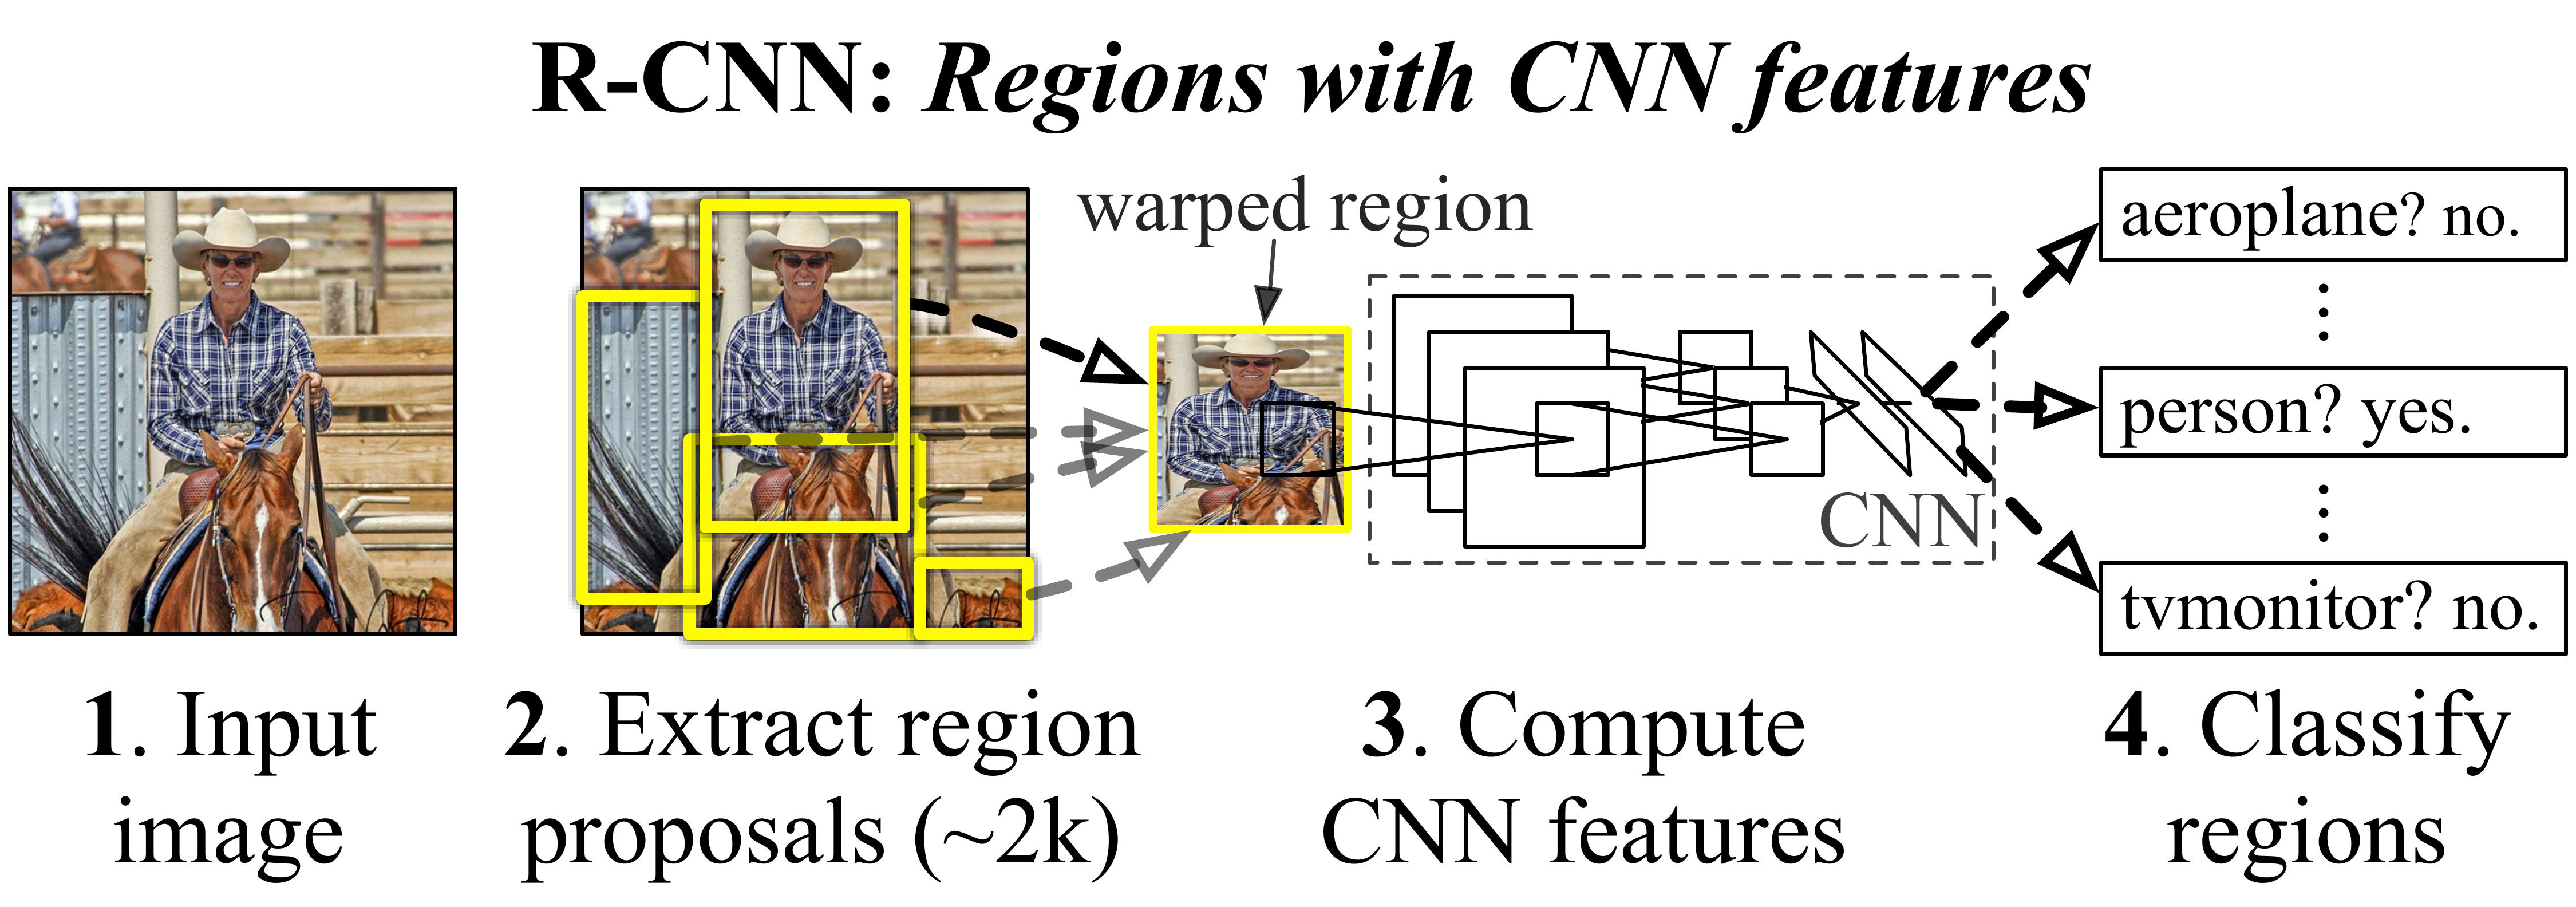
\includegraphics[width=0.70\linewidth]{fig/R-CNN.jpg}
 	\caption{R-CNN}
 	\label{fig:r-cnn}
\end{figure}
 
R-CNN is een trage detector vermits elke RoIs door een CNN moet gaan. Deze methode is ge\"evolueerd tot de veel snellere methode Faster R-CNN (figuur \ref{fig:faster-r-cnn}). Hierbij wordt de afbeelding door een CNN behandelt en vervolgens maakt men gebruik van een Region Proposal Network (RPN). Het RPN gaat zoals bij R-CNN regios uit de afbeelding filteren waar de kans groot is dat er objecten opstaan, maar het RPN werkt sneller en levert betere resultaten. 
%dieper op RPN ingaan?

\begin{figure}[!ht]
    \centering
 	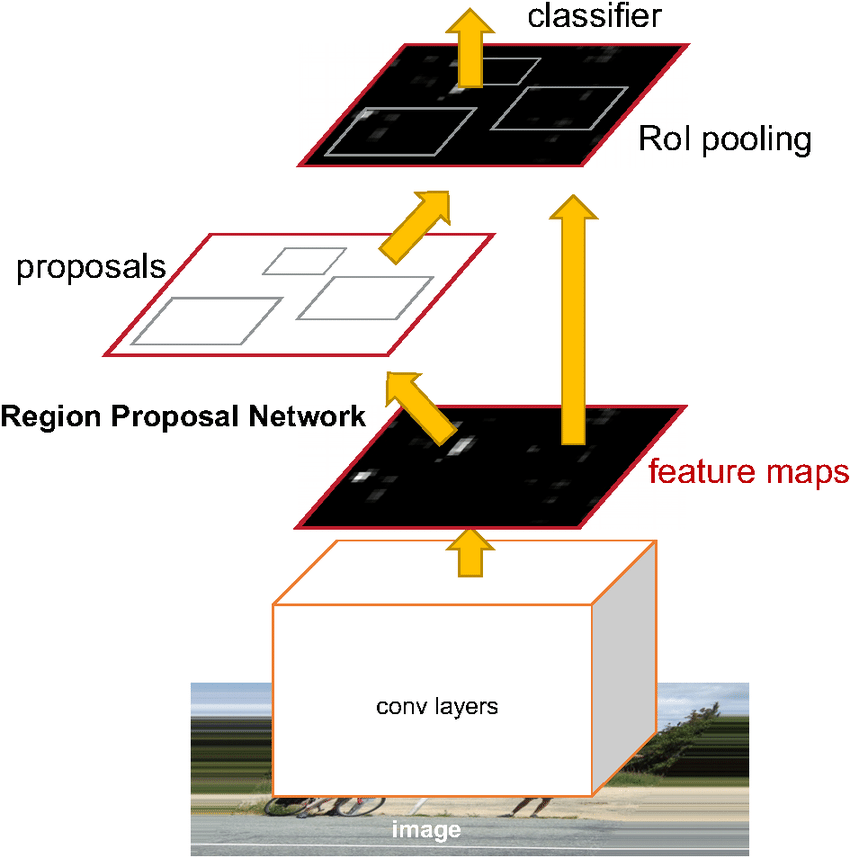
\includegraphics[width=0.3\linewidth]{fig/Faster-R-CNN.png}
 	\caption{Faster R-CNN}
 	\label{fig:faster-r-cnn}
\end{figure}

\begin{enumerate}
    \item CNN waarbij men eerst features uit de afbeelding haalt
    \item RPN waarbij een netwerk op basis van de features RoIs genereert
    \item RoI pooling 
    \item Classificatie en regresie laag: verfijnt de posities van de RoIs
\end{enumerate}

\subsection{One-stage detector}
Bij one-stage detectoren gebeurt object detectie in \'e\'en keer met \'e\'en neuraal netwerk. Dus er is geen region proposal niveau meer zoals bij de two-stage detector (figuur \ref{fig:ssd}). One-stage detectoren zijn sneller dan two-stage detectoren omdat ze alles in \'e\'en keer doen, maar kunnen wat in nauwkeurigheid verliezen t.o.v. two-stage detectroren.

\begin{figure}[!ht]
 	\centering
 	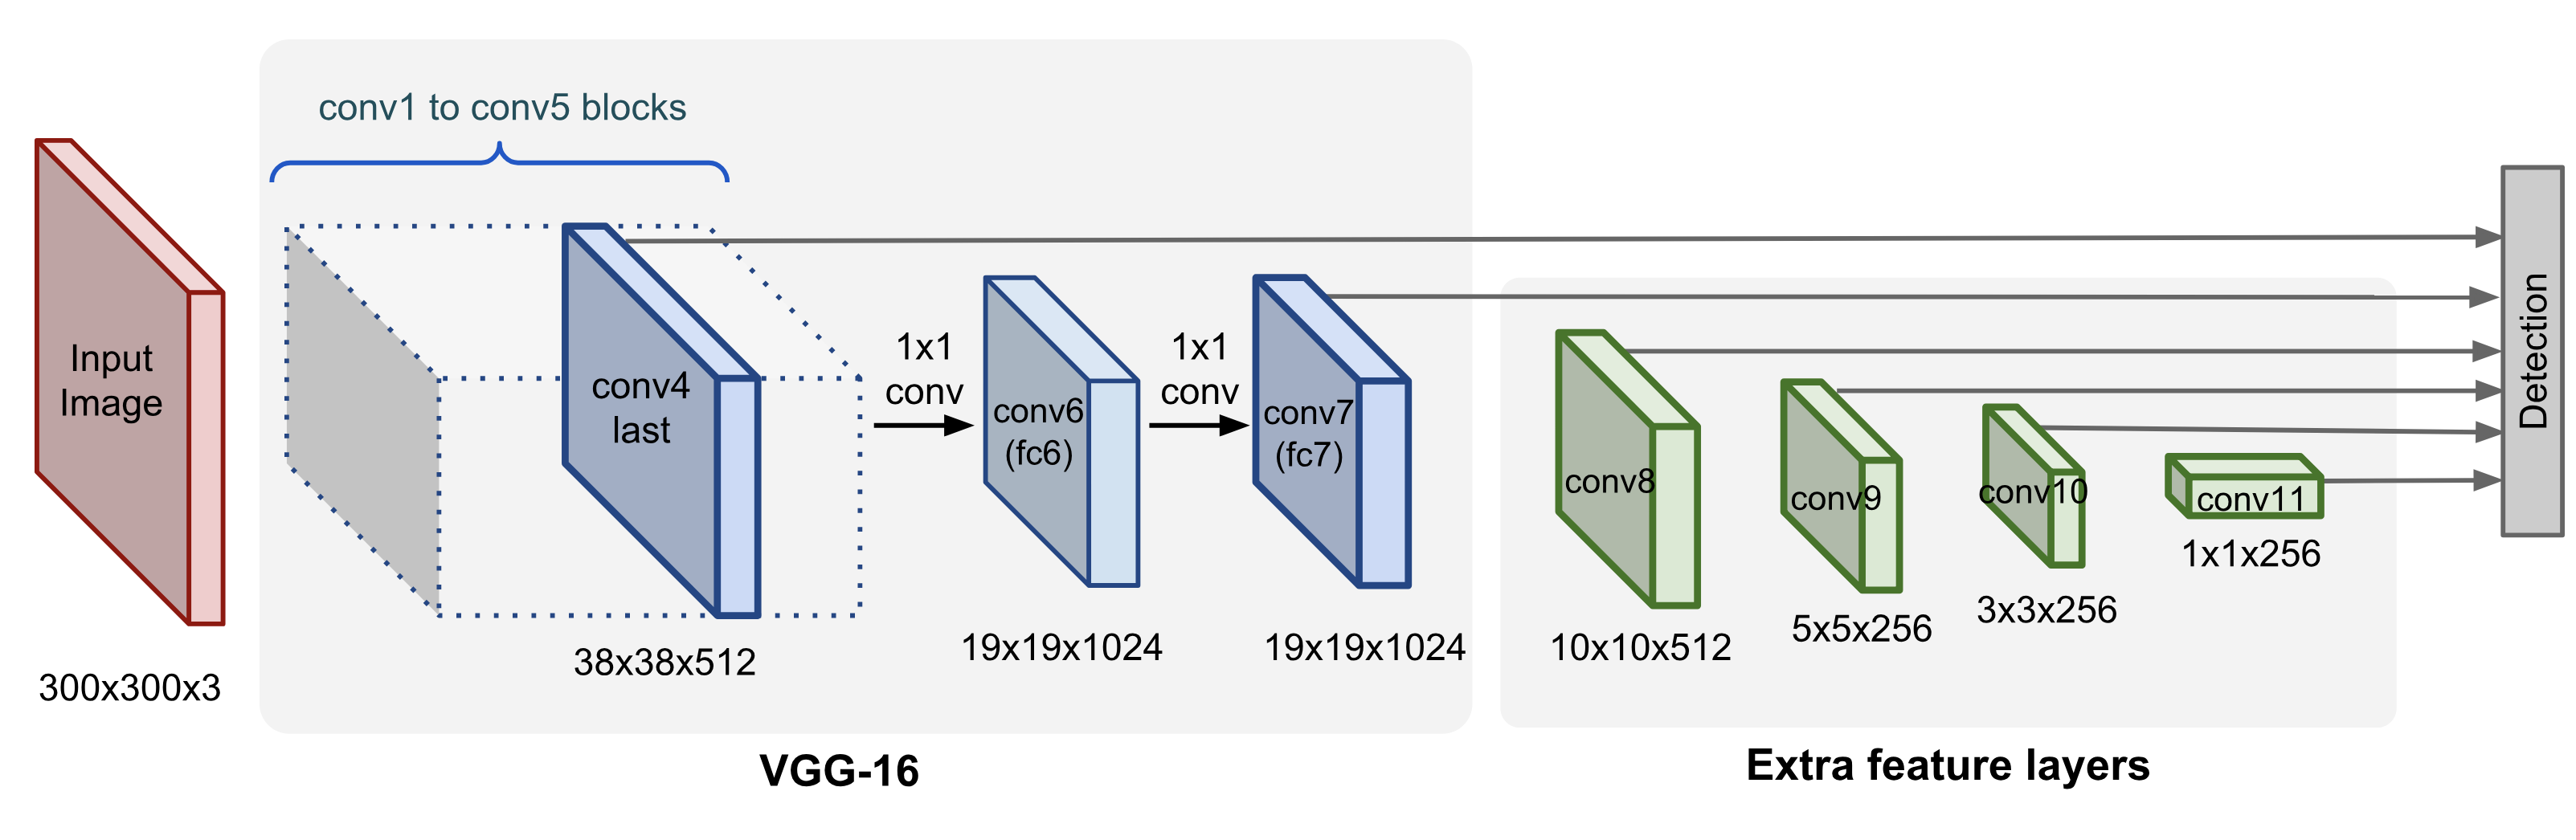
\includegraphics[width=0.80\linewidth]{fig/SSD.png}
 	\caption{One-stage detector met VGG net backbone}
 	\label{fig:ssd}
\end{figure}
 
One-stage detectie netwerken bestaat uit 2 delen: een backbone en 1 of meerder convolutie lagen. De backbone van het netwerk is een getraind CNN classificatie netwerk dat de als feature extractor dient. Dit is een CNN waarvan de fully-connected lagen zijn weggelaten in figuur \ref{fig:ssd} vormt VGG de backbone van de single-stage detector. De extra convolutie lagen gaan de objecten detecteren op basis van de feature mappen die de output zijn van de backbone. 

De input afbeelding wordt opgedeeld in een rooster, voor elke cel van het rooster gaat men de klasse en locatie van het object voorspellen. Als er geen object is wordt de cel gezien als een achtergrond klasse. Voor elke locatie van een object wordt er een vaste set van anchor/bounding boxen ge\"evalueren. Vervolgens is er nog een methode nodig voor de overbodige bounding boxen te verwijderen. Een eerste mogelijkheid is door enkel bounding boxen te tekenen waarvan de voorspelling boven een treshold ligt. Een andere methode is non-maxima supression deze methode zorgt ervoor dat elk object maar \'e\'en bounding box heeft.  Deze techniek houdt enkel de bounding box over met de beste voorspelling en onderdrukt de rest van de bounding boxen. 
%via IoU, uitleggen?
De twee bekenste technieken van one-stage detectie zijn: You Only Look Once (YOLO) en Single Shot Detection (SSD).

\chapter{Herkenning en detectie implementatie op mobiel platform}
